\subsection*{Results and Discussion}

After fitting the models 30 times, we consider the models with a loss equal to at most 1.0005 times the loss of the best model.
There are two models (apart from the best model) with low enough losses to be considered, and their match scores compared with the best model for each of the three datasets are shown in Table \ref{tab:score} below.

\begin{table}[H]
    \centering
    \begin{tabular}{|c|c|c|}
         \hline
         $\ten{X}$ & $\ten{Y}$ & $Z$ \\
         \hline
         0.9996 & 0.9997 & 0.9959 \\
         \hline
         1.0000 & 1.0000 & 0.9731 \\
         \hline
    \end{tabular}
    \caption{FMS scores for second and third best models compared to best model.}
    \label{tab:score}
\end{table}

We see that the factors for every part of the dataset have FMS scores close to 1, demonstrating that models with loss close to the best model also have their factors close to the best model.
This demonstrates uniqueness: we do not obtain models of similar performance to the best one with vastly different sets of factors.

All factors from the CMTF-analysis are plotted in Figure \ref{fig:fac2} (EEM and NMR) and Figure \ref{fig:fac3} (LC-MS).
We notice that the factors of the EEM part in Figure \ref{fig:fac2} closely resemble those in Figure \ref{fig:plot_factors}.
This is to be expected, as they model the same data.
Furthermore, we see that the first three factors are identical in the first mode over all three plots, as well as the fourth factor (yellow line) being identical in the first mode for NMR and LC-MS plots.
This confirms that our couplings works as expected.

As in part 1, we can identify the underlying properties of each chemical contained in the mixtures by studying the plots.
Indeed, the chemical shifts, gradient levels, and features of each of the chemicals are shown in Figures \ref{fig:fac2} and \ref{fig:fac3}.

Note that the relative sizes of the factors are slightly different between Figures \ref{fig:plot_factors} and \ref{fig:fac2}, since the factors in Figure \ref{fig:fac2} are not normalized.
When comparing, we are only interested in the shapes of the graphs, not the absolute size.

\begin{figure}[H]
    \centering
    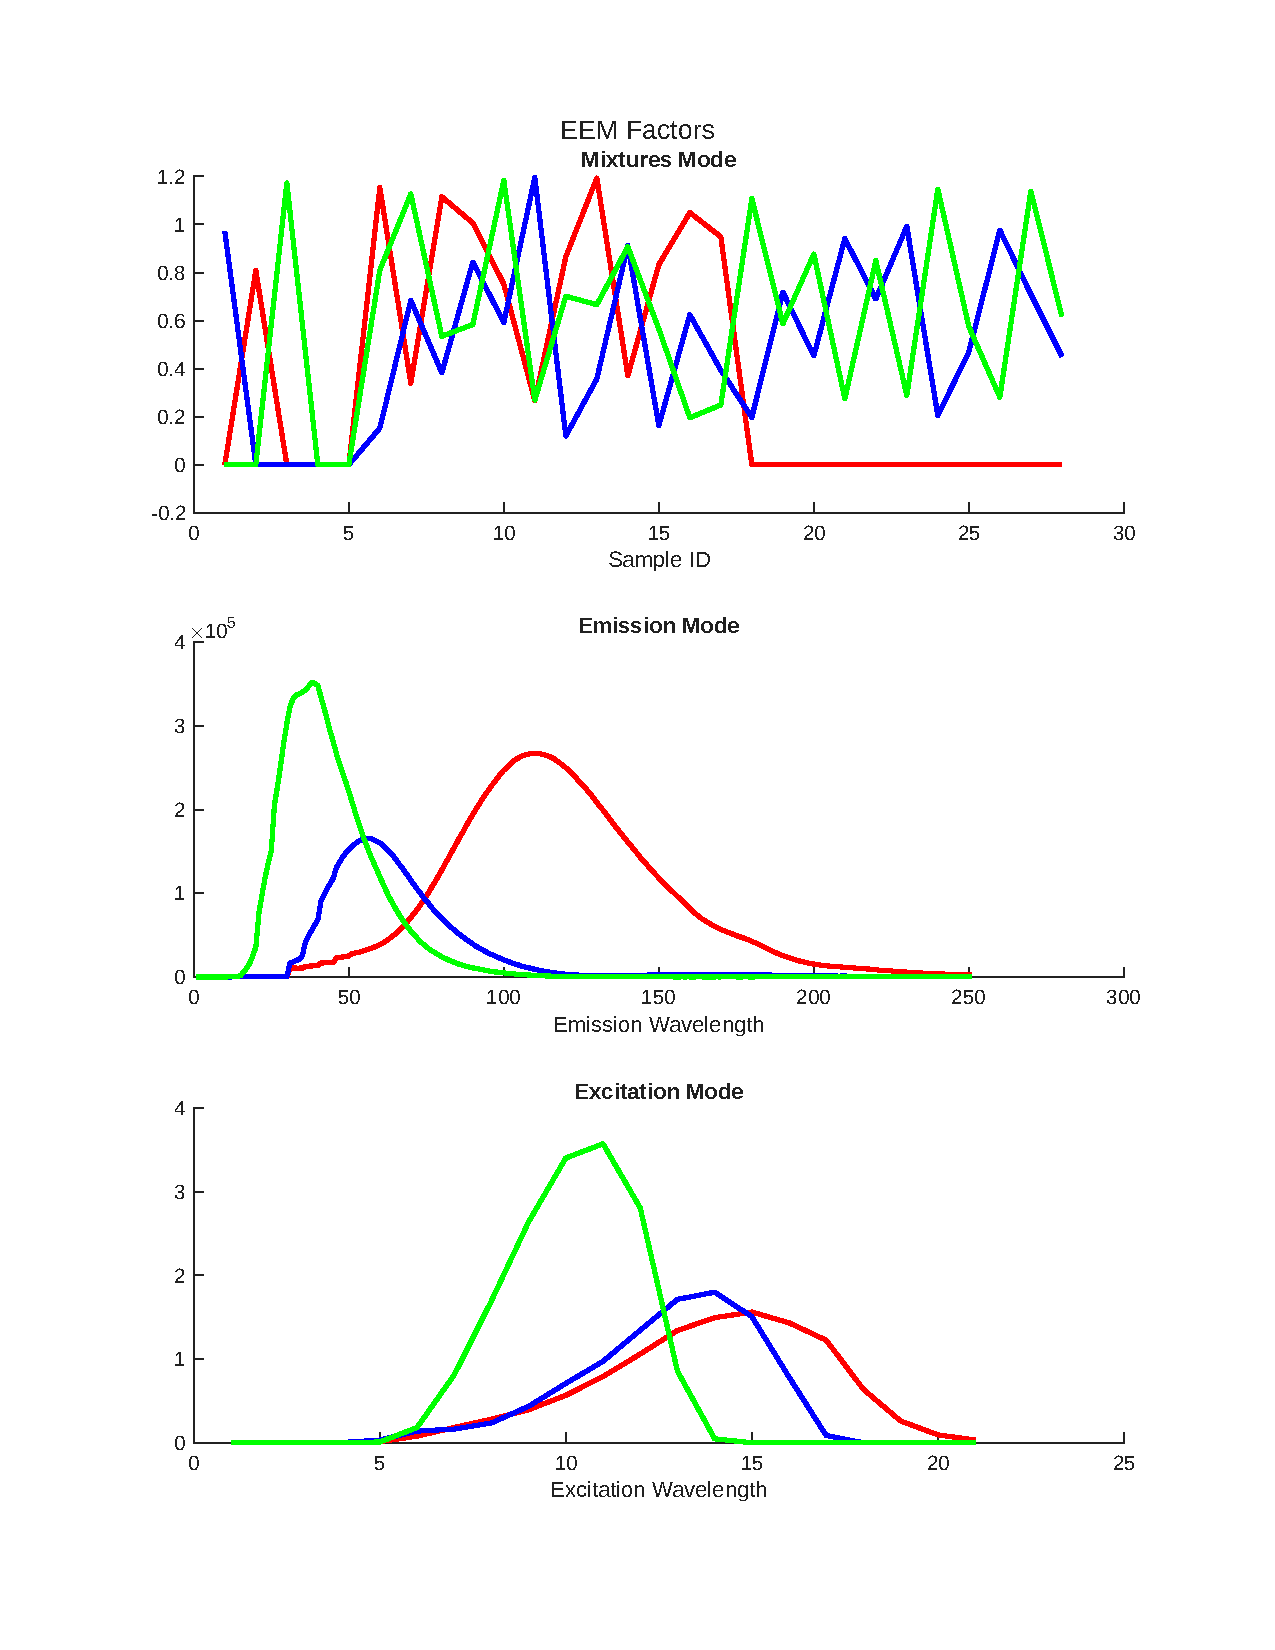
\includegraphics[trim = 2cm 2.5cm 2cm 1.9cm, clip, width=0.46\linewidth]{figures/factors_EEM Factors.pdf}
    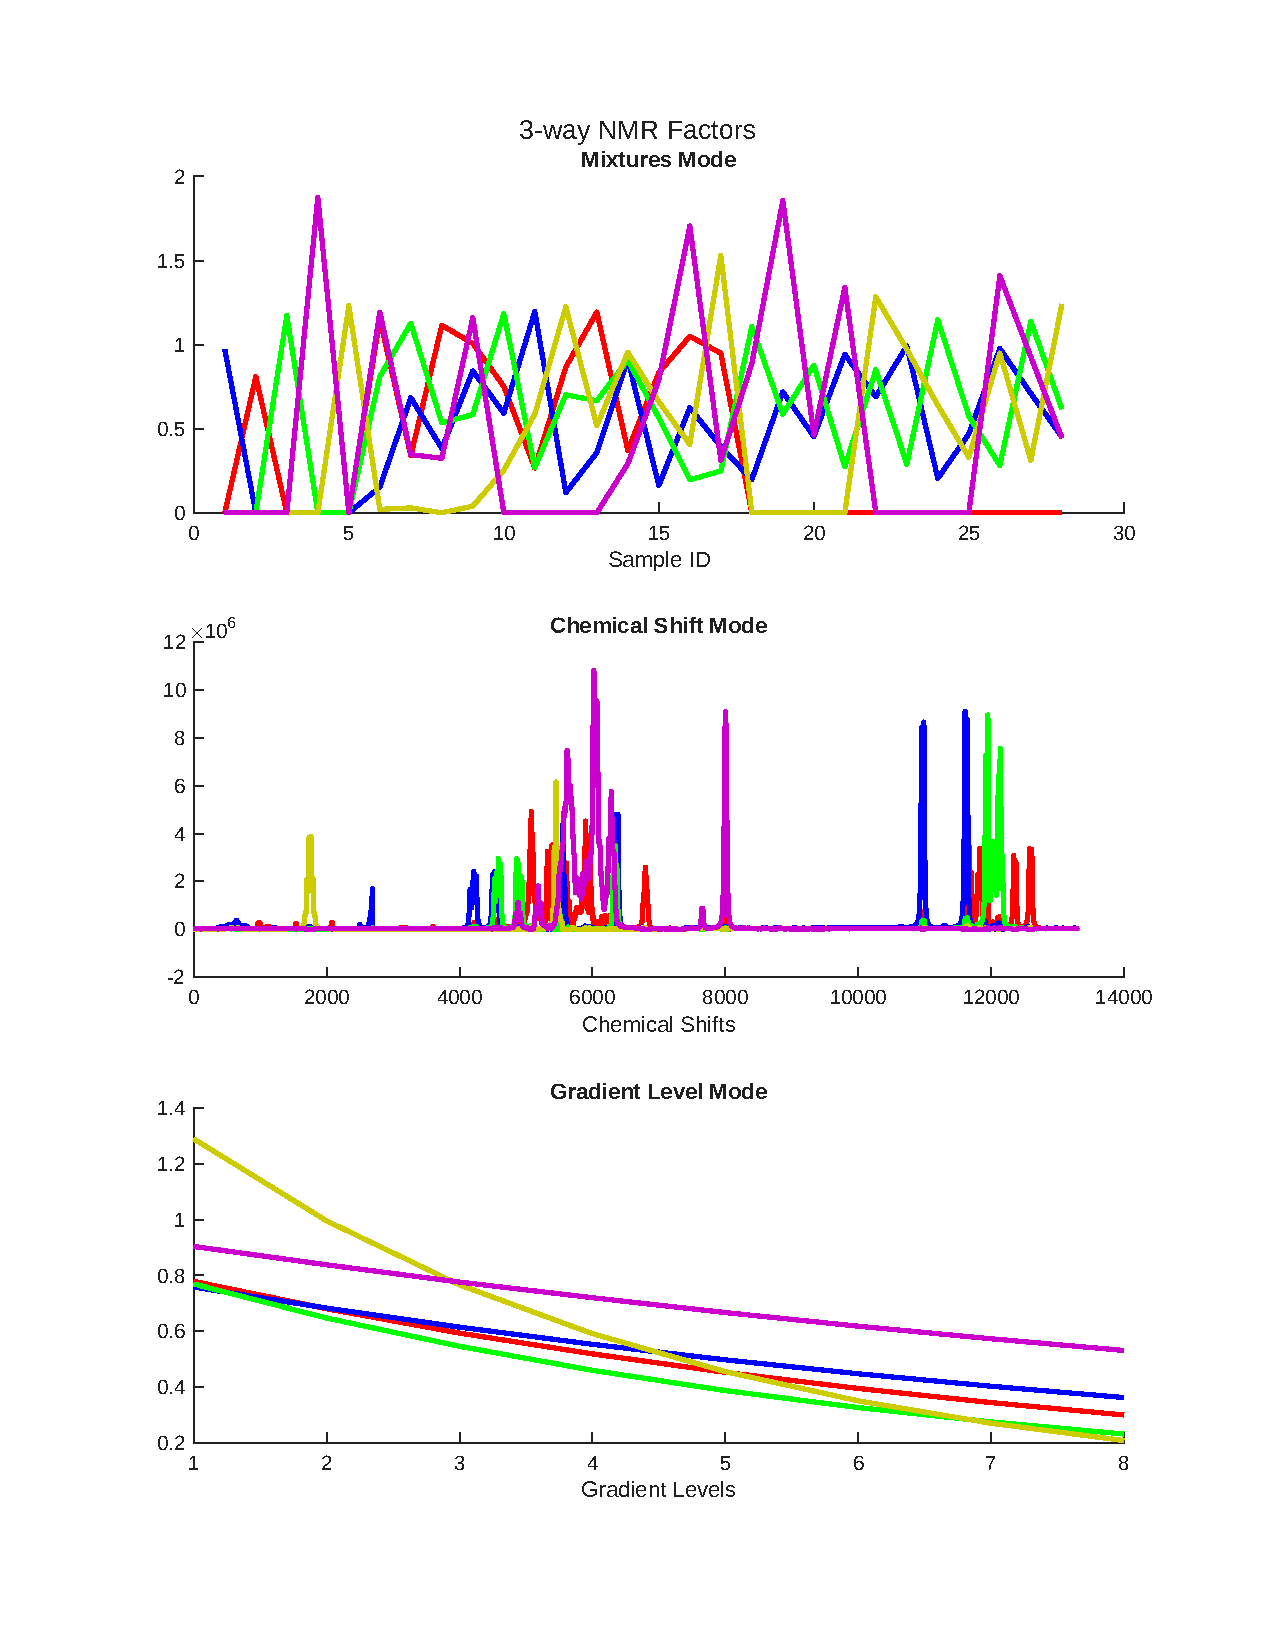
\includegraphics[trim = 2cm 2.5cm 2cm 1.9cm, clip, width=0.46\linewidth]{figures/factors_3-way NMR Factors.pdf}
    \caption{Discovered factors for EEM and NMR data}
    \label{fig:fac2}
\end{figure}
\begin{figure}[H]
    \centering
    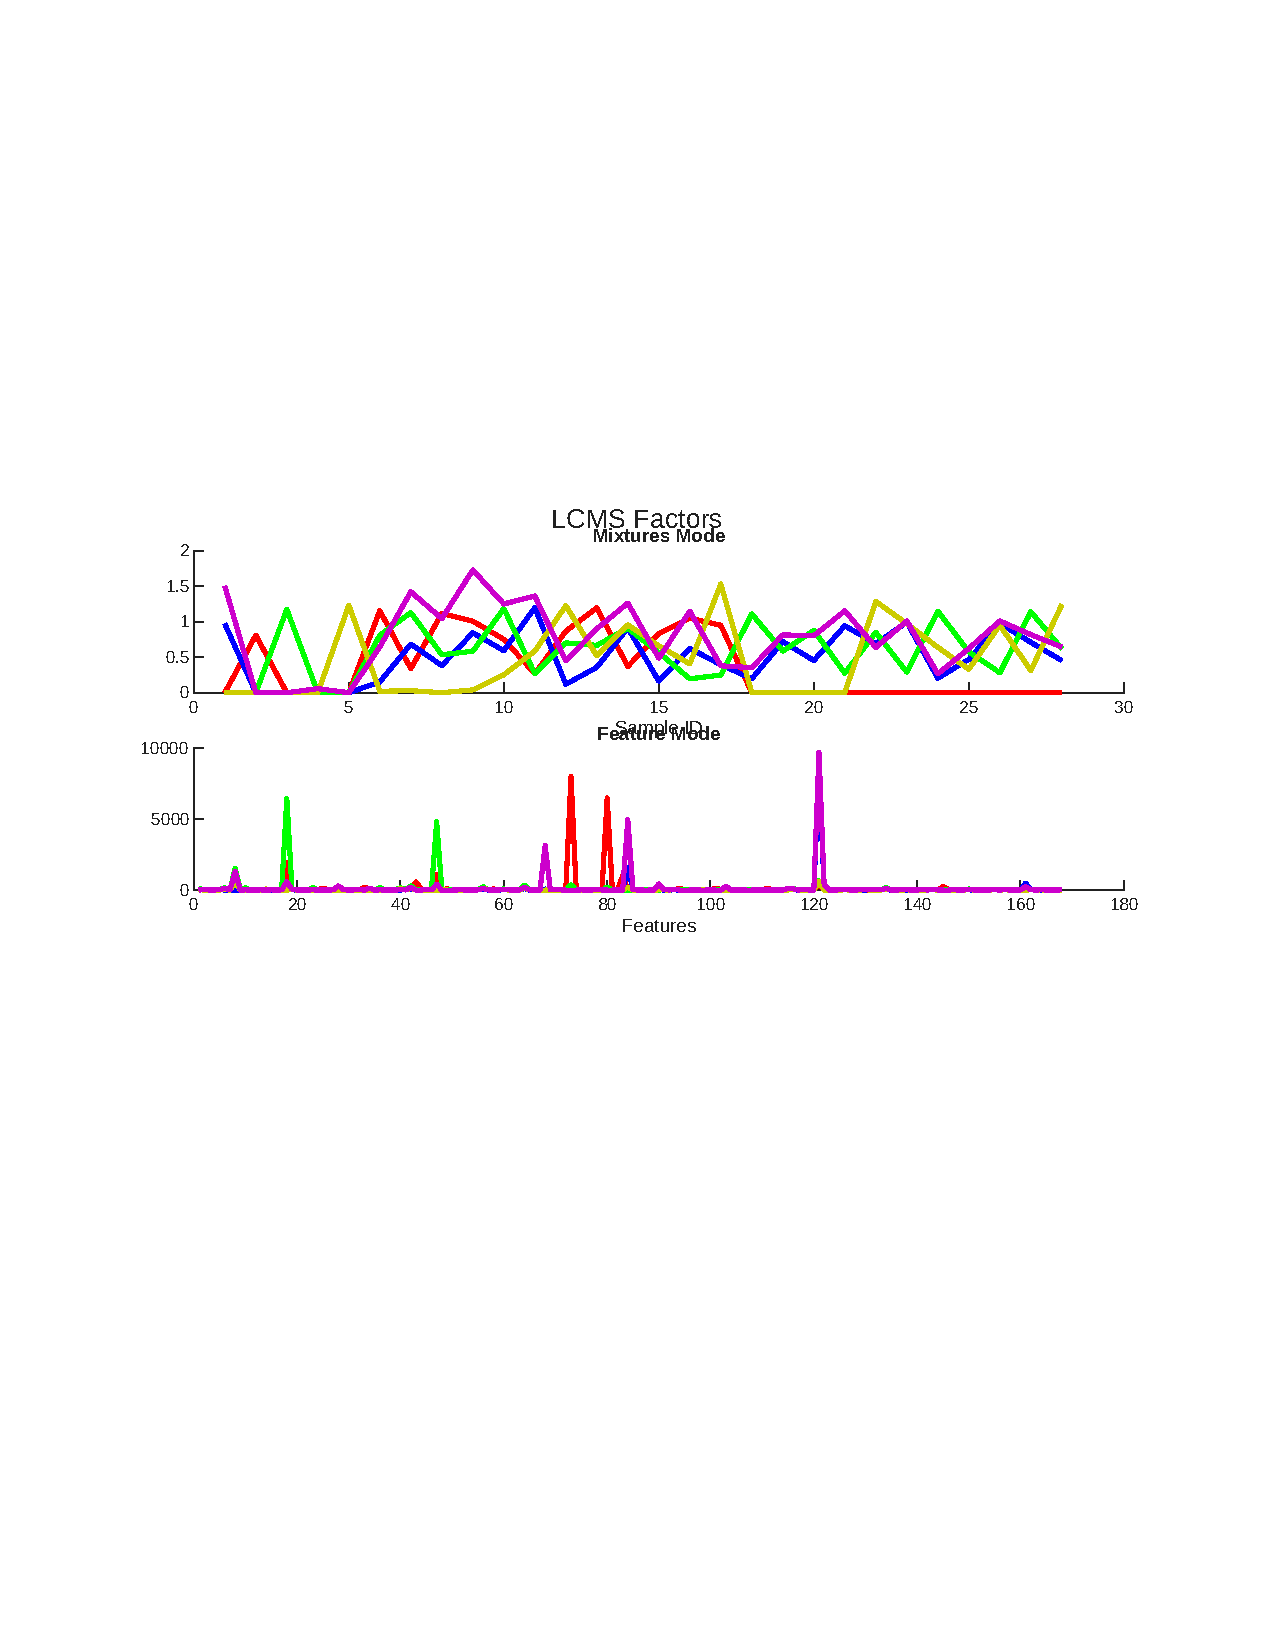
\includegraphics[trim = 2cm 10cm 2cm 1.9cm, clip, width=0.46\linewidth]{figures/factors_LCMS Factors.pdf}
    \caption{Discovered factors for LC-MS data.}
    \label{fig:fac3}
\end{figure}
